\documentclass{beamer}
\usepackage[utf8]{inputenc}
\usepackage{amsmath}
\usepackage{amssymb,latexsym,amsmath,epsfig,amsthm}
\usepackage{qrcode}
\usepackage{graphicx}
\graphicspath{ {./assets/} }

\usetheme{Madrid} \usecolortheme{beaver}

\title{Transformation Matricies}

\subtitle{Unit 1 Assessment}

\author{Lucien Gaitskell}
\date{October 2020}

\begin{document}

\maketitle

\begin{frame}{My Project}

So\dots \pause

\large You probably can assume what form my project is going to take.

\end{frame}

\begin{frame}{The essential question}
  
  \begin{center}
    \Huge WHY? \pause

    \Large Why a computer science application?
  \end{center}

\end{frame}

\begin{frame}{Computer Graphics}
  \begin{center}
    \LARGE I'm not the only one!
  
    \vspace{5mm}

    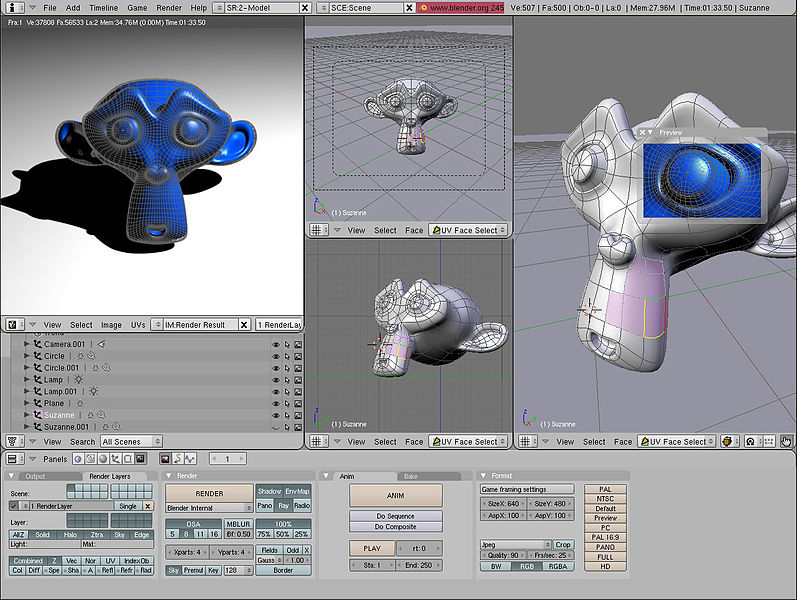
\includegraphics[scale=0.18]{monkey}
    
\includegraphics[scale=0.08]{vector1}
  \end{center}
\end{frame}

\begin{frame}{Starting Simple}

  How would you represent even simple changes?

  \vspace{5mm}

  \begin{center}
    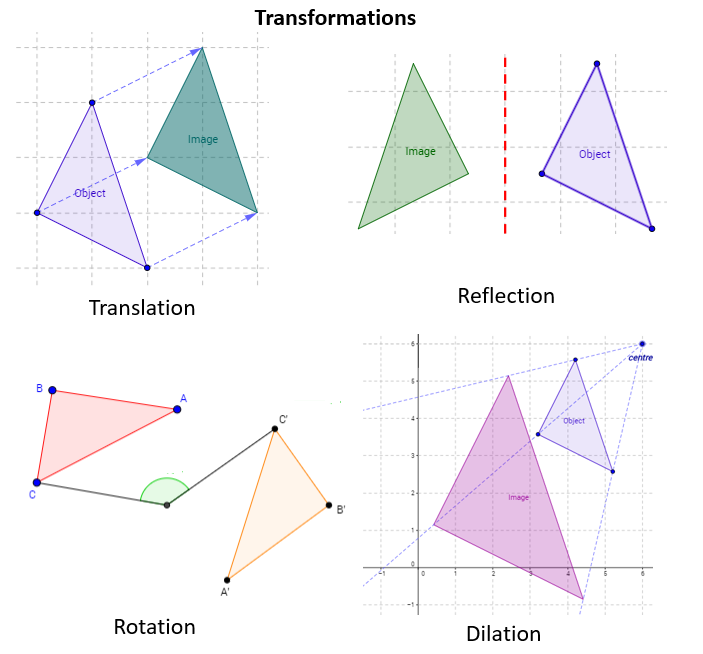
\includegraphics[height=6cm]{transformations}
  \end{center}

\end{frame}

\begin{frame}{Scaling}

  \begin{center}
    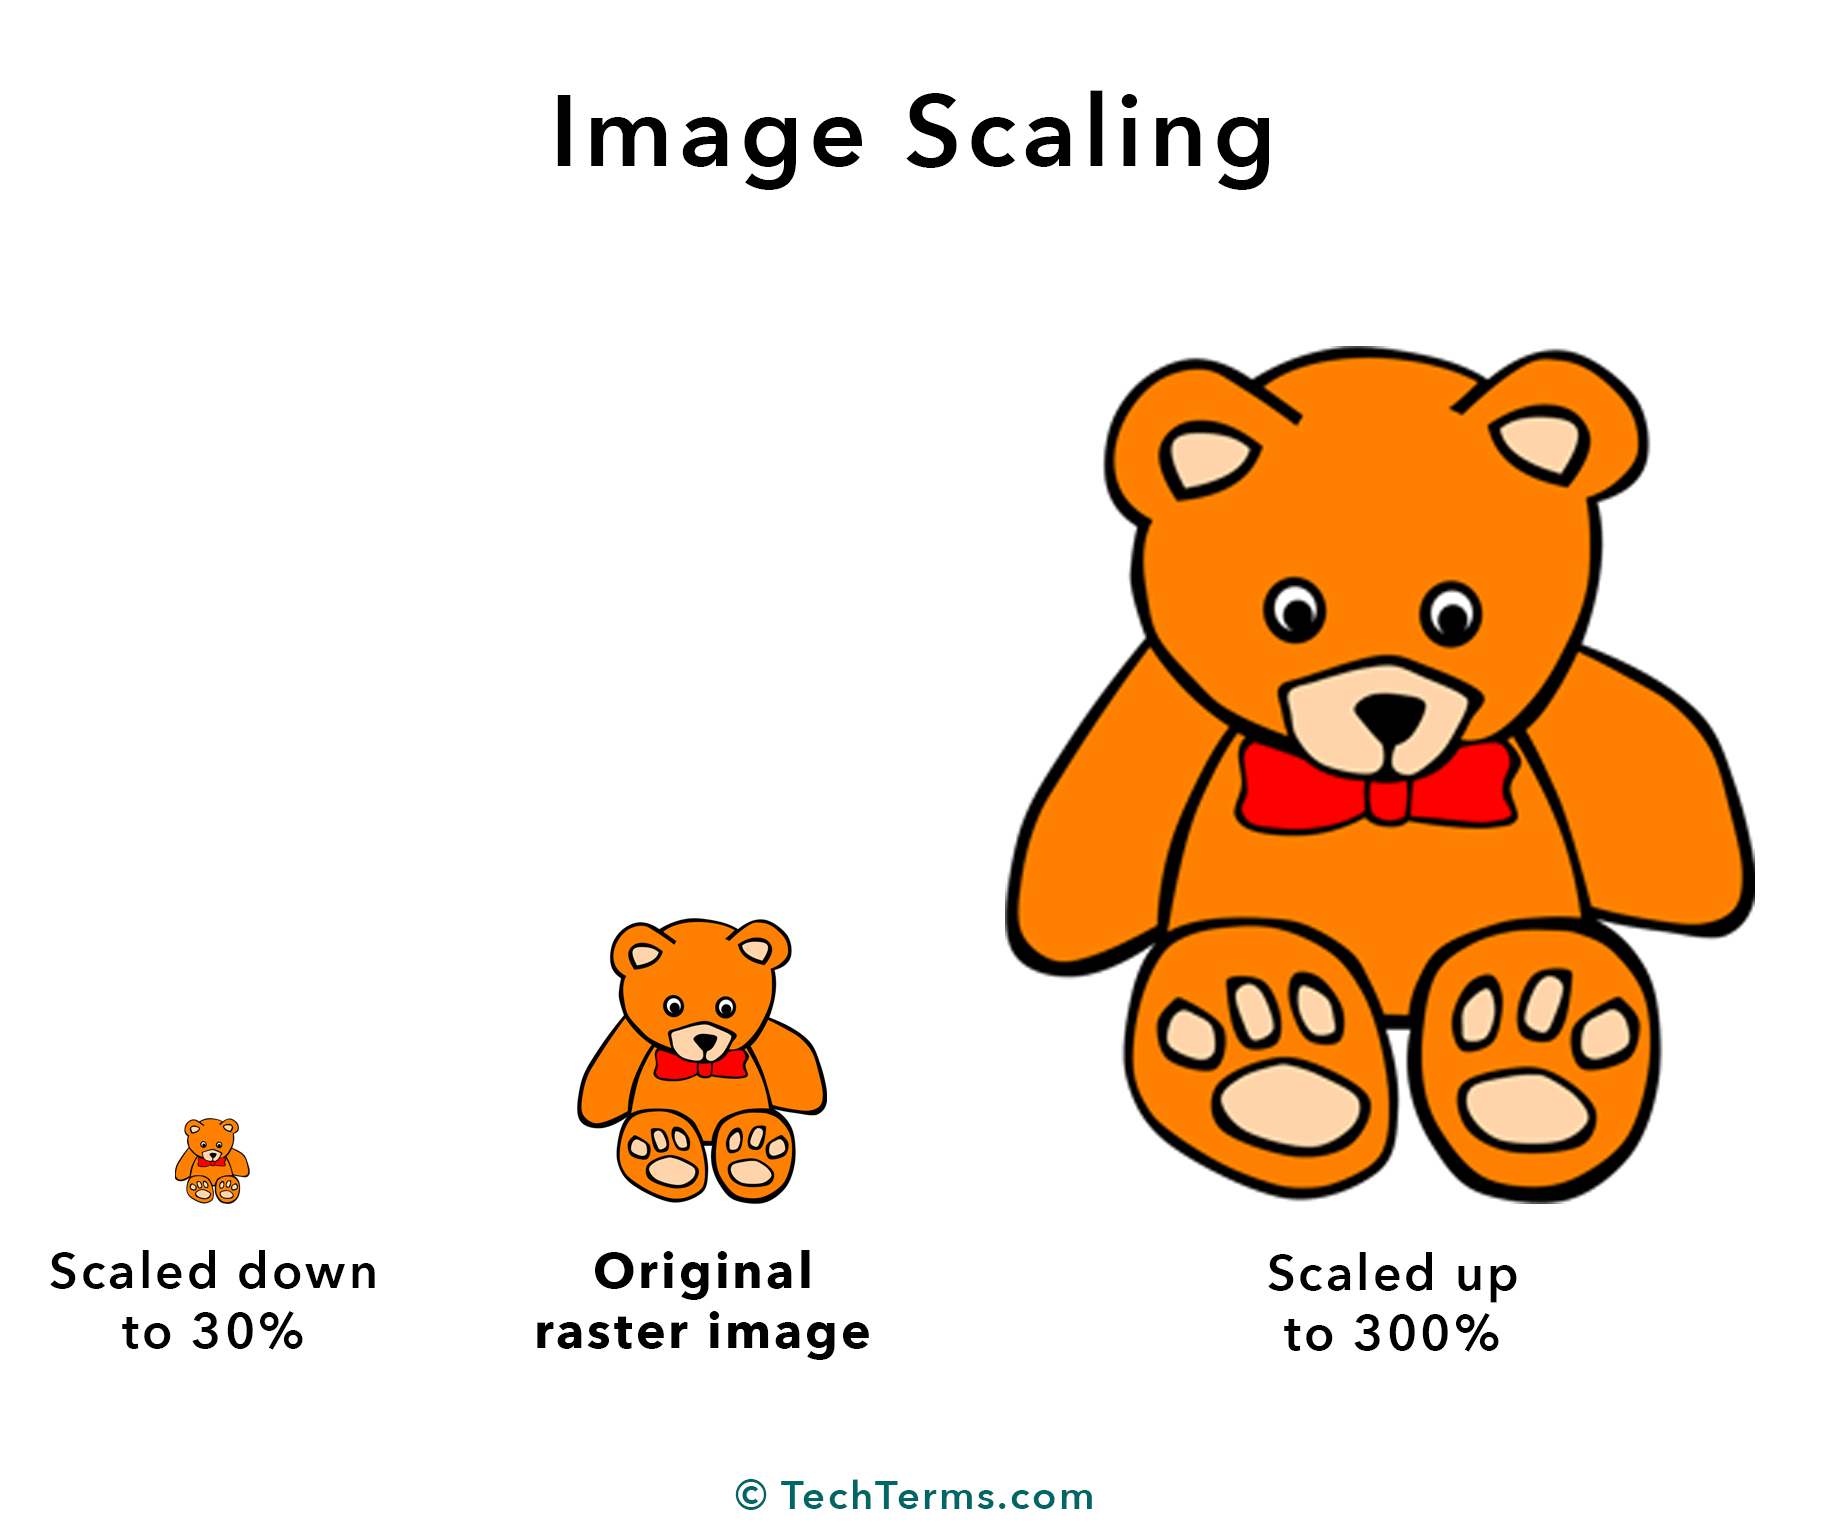
\includegraphics[height=4cm]{scale}
  \end{center} \pause


  \[
    \begin{bmatrix}
      a & 0 \\
      0 & b
    \end{bmatrix}
    \cdot
    \begin{bmatrix}
      x \\ y
    \end{bmatrix}
    = \pause
    \begin{bmatrix}
      ax \\ by
    \end{bmatrix}
  \]
  \pause

  Therefore $a$ is the scale factor for x and $b$ is the scale factor for y.

\end{frame}

\begin{frame}{Shear}

  \begin{center}
    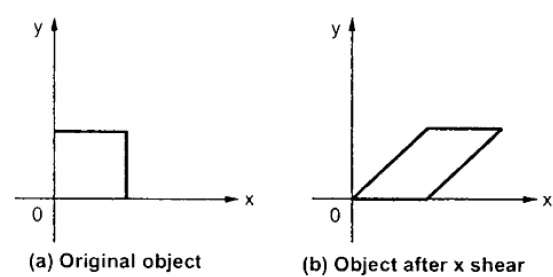
\includegraphics[height=2cm]{shear_x}
  \end{center} \pause

  \begin{block}{Definition}
    A matrix shear is the addition of one row/column, multiplied by some factor, to another row/column.
  \end{block} \pause

  {\Large Thus:} \pause

  \[
    \begin{bmatrix}
      1 & k \\
      j & 1
    \end{bmatrix}
    \cdot
    \begin{bmatrix}
      x \\ y
    \end{bmatrix}
    =
    \begin{bmatrix}
      x + ky \\ jx + y
    \end{bmatrix}
  \] \pause

  Therefore $k$ is the shear parallel to the $x$ axis, while $j$ is the shear parallel to the $y$ axis. 

\end{frame}

\begin{frame}{Rotation}
  
  \begin{center}
    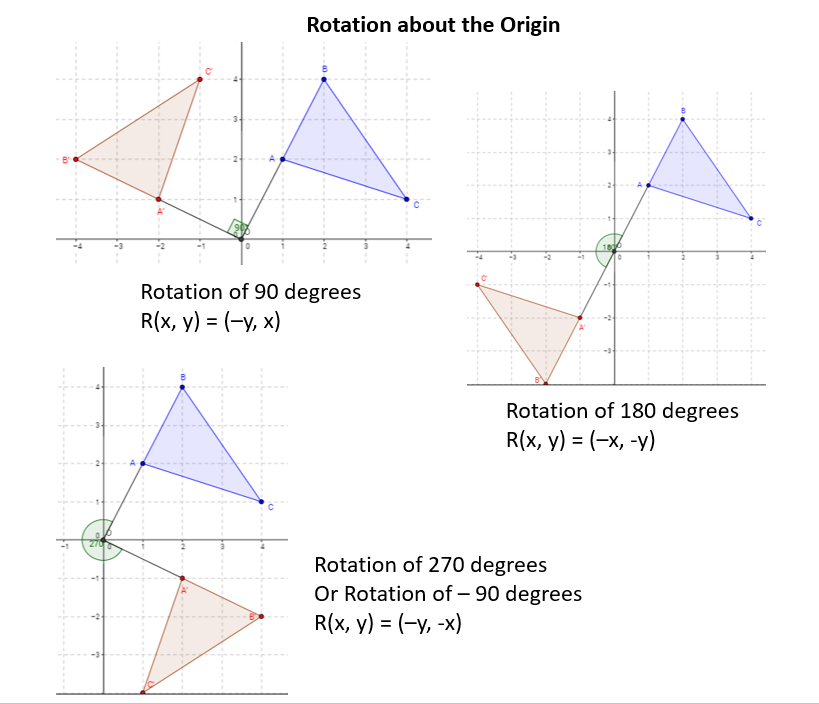
\includegraphics[height=6cm]{rotation}
  \end{center}
  
\end{frame}

\begin{frame}{Rotation}{Around the origin}

  \begin{columns}
    \begin{column}{0.3\textwidth}
      It's just like polar! \pause
    \end{column}
    \begin{column}{0.7\textwidth}
      \begin{align*}
        x = r\cos{\phi} \\
        y = r\sin{\phi}
      \end{align*} \pause
    \end{column}
  \end{columns}

  \begin{columns}
    \begin{column}{0.3\textwidth}
      Let's add the rotation: \pause
    \end{column}
    \begin{column}{0.7\textwidth}
      \begin{align*}
        x^{\prime} = r\cos{(\phi + \theta)} \\
        y^{\prime} = r\sin{(\phi + \theta)}
      \end{align*} \pause
    \end{column}
  \end{columns}

  
  \begin{columns}
    \begin{column}{0.3\textwidth}
      Expand: \pause
    \end{column}
    \begin{column}{0.7\textwidth}
      \begin{align*}
        x^{\prime} = r(\cos{(\phi)}\cos(\theta) - \sin{(\phi)}\sin(\theta)) \\
        y^{\prime} = r(\sin{(\phi)}\cos(\theta) + \cos{(\phi)}\sin(\theta))
      \end{align*} \pause
    \end{column}
  \end{columns}

\end{frame}

\begin{frame}{Rotation}{into a matrix}

  \begin{columns}
    \begin{column}{0.3\textwidth}
      Expand: \pause
    \end{column}
    \begin{column}{0.7\textwidth}
      \begin{align*}
        x^{\prime} = r\cos{(\phi)}\cos(\theta) - r\sin{(\phi)}\sin(\theta) \\
        y^{\prime} = r\sin{(\phi)}\cos(\theta) + r\cos{(\phi)}\sin(\theta)
      \end{align*} \pause
    \end{column}
  \end{columns}

  \begin{columns}
    \begin{column}{0.3\textwidth}
      Substitute: \pause
    \end{column}
    \begin{column}{0.7\textwidth}
      \begin{align*}
        x^{\prime} &= x\cos(\theta) - y\sin(\theta) \\
        y^{\prime} &= y\cos(\theta) + x\sin(\theta) \\
                   &= x\sin(\theta) + y\cos(\theta)
      \end{align*} \pause
    \end{column}
  \end{columns}


  \[
    \begin{bmatrix}
      \cos{\theta} & -\sin{\theta} \\
      \sin{\theta} & \cos{\theta}
    \end{bmatrix}
    \cdot
    \begin{bmatrix}
      x \\ y
    \end{bmatrix}
    = \pause
    \begin{bmatrix}
      x\cos{\theta} - y\sin{\theta} \\
      x\sin{\theta} + y\cos{\theta}
    \end{bmatrix}
  \]

\end{frame}

\begin{frame}{So what did I do?}
  
  \begin{center}
    \huge I made a website!

    \vspace{1cm}

    \qrcode[height=1in]{https://linear-luc.herokuapp.com}

  \end{center}

\end{frame}

\begin{frame}{Let's combine everything}
  
  \begin{enumerate}
    \item Scaling\pause
    \item Shear\pause
    \item Rotation\pause
  \end{enumerate}

  \vspace{1cm}

  \[
    \begin{bmatrix}
      a & 0 \\
      0 & b
    \end{bmatrix}\pause
    \cdot
    \begin{bmatrix}
      1 & k \\
      j & 1
    \end{bmatrix}\pause
    \cdot
    \begin{bmatrix}
      \cos{\theta} & -\sin{\theta} \\
      \sin{\theta} & \cos{\theta}
    \end{bmatrix}
  \]
\end{frame}

\begin{frame}{Example}{starting simple}
  \begin{columns}
    \begin{column}{0.6\textwidth}
      {\Large How do you rotate an object 90° around the axis?} \pause

      \vspace{10mm}

      angle: $\theta$; shear: ($j, k$); scale: ($a, b$)
    \end{column}

    \begin{column}{0.4\textwidth}
      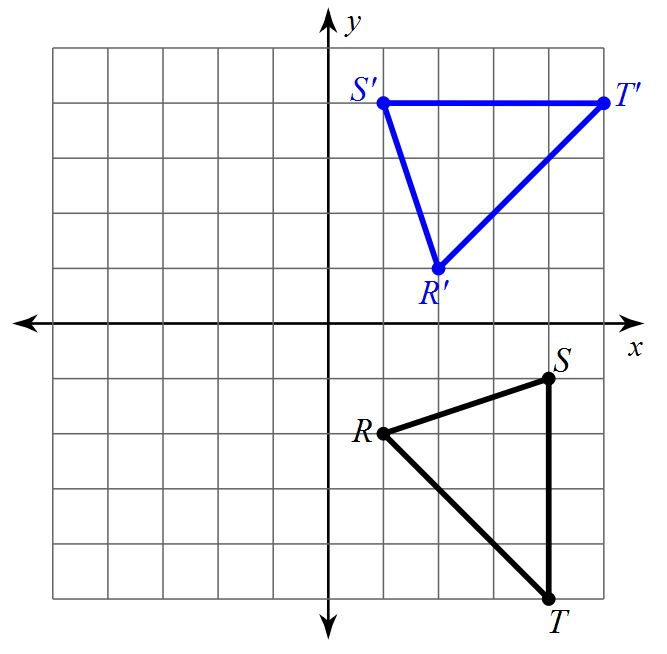
\includegraphics[height=30mm]{example_rotation}
    \end{column}

  \end{columns}
  

  \vspace{0.5cm}

  \begin{columns}
    \begin{column}{0.3\textwidth}
      \begin{align*}
        \theta &= 90^{\circ} \\
        a &= 1 \\
        b &= 1 \\
        j &= 0 \\
        k &= 0
      \end{align*} \pause
    \end{column}
    \begin{column}{0.7\textwidth}
      \begin{align*}
        \begin{bmatrix}
          1 & 0 \\
          0 & 1
        \end{bmatrix}
        \cdot
        \begin{bmatrix}
          1 & 0 \\
          0 & 1
        \end{bmatrix}
        \cdot
        \begin{bmatrix}
          \cos{90^{\circ}} & -\sin{90^{\circ}} \\
          \sin{90^{\circ}} & \cos{90^{\circ}}
        \end{bmatrix}
        =
        \begin{bmatrix}
          0 & -1 \\
          1 & 0
        \end{bmatrix}
      \end{align*}
    \end{column}
  \end{columns}
\end{frame}

\begin{frame}{Example}{harder}

  {\Large How do you rotate a shape 37° around the axis, and shear by a factor of
          0.5 in the $x$ axis, while also scaling the $y$ axis by 3?} \pause
      
  Try and visualize that... \pause

  angle: $\theta$; shear: ($j, k$); scale: ($a, b$)

  \vspace{1cm}

  \begin{columns}
    \begin{column}{0.3\textwidth}
      \begin{align*}
        \theta &= 37^{\circ} \\
        a &= 1 \\
        b &= 3 \\
        j &= 0 \\
        k &= 0.5
      \end{align*} \pause
    \end{column}
    \begin{column}{0.7\textwidth}
      \begin{align*}
        \begin{bmatrix}
          1 & 0 \\
          0 & 3
        \end{bmatrix}
        \cdot
        \begin{bmatrix}
          1 & 0.5 \\
          0 & 1
        \end{bmatrix}
        \cdot
        \begin{bmatrix}
          \cos{37^{\circ}} & -\sin{37^{\circ}} \\
          \sin{37^{\circ}} & \cos{37^{\circ}}
        \end{bmatrix} \\
        =
        \begin{bmatrix}
          1.099 & -0.202 \\
          1.805 & 2.396
        \end{bmatrix}
      \end{align*}
    \end{column}
  \end{columns}
\end{frame}

\begin{frame}{Computer Science}{back again...}

  \begin{center}
    \huge Try out the site!

    \vspace{1cm}

    \qrcode[height=1in]{https://linear-luc.herokuapp.com}

  \end{center}

\end{frame}

\end{document}
